\begin{figure}[h!]
    \centering
    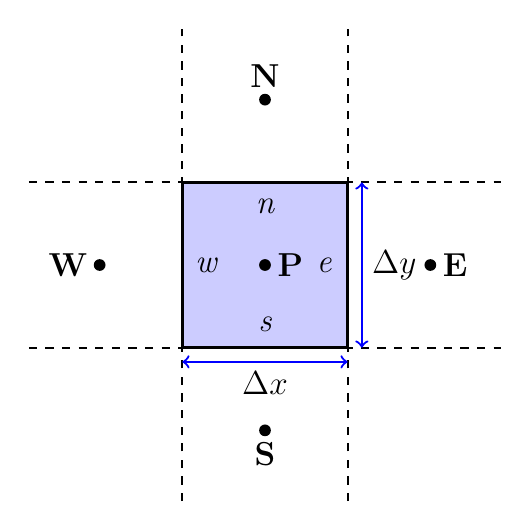
\begin{tikzpicture}[
        scale=0.6,
        font=\large,
        cv_node/.style={
            fill=black, 
            circle, 
            inner sep=1.5pt
        },
        node_label/.style={
            font=\large\bfseries,
            inner sep=2pt
        },
        face_label/.style={
            font=\large\itshape,
            inner sep=1pt
        }
    ]
        \def\nodedist{3.5cm}
        \def\grid_extent{5cm}
        
        \draw[dashed, line width=0.8pt] (-\grid_extent, \nodedist/2) -- (\grid_extent, \nodedist/2);
        \draw[dashed, line width=0.8pt] (-\grid_extent, -\nodedist/2) -- (\grid_extent, -\nodedist/2);
        \draw[dashed, line width=0.8pt] (\nodedist/2, -\grid_extent) -- (\nodedist/2, \grid_extent);
        \draw[dashed, line width=0.8pt] (-\nodedist/2, -\grid_extent) -- (-\nodedist/2, \grid_extent);

        \draw[line width=1.0pt, fill=blue!20] 
            (-\nodedist/2, -\nodedist/2) rectangle (\nodedist/2, \nodedist/2);
        
        \node[cv_node, label={[node_label]right:P}] (P) at (0,0) {};
        \node[cv_node, label={[node_label]above:N}] (N) at (0, \nodedist) {};
        \node[cv_node, label={[node_label]below:S}] (S) at (0, -\nodedist) {};
        \node[cv_node, label={[node_label]right:E}] (E) at (\nodedist, 0) {};
        \node[cv_node, label={[node_label]left:W}] (W) at (-\nodedist, 0) {};
        
        \node[face_label] at (\nodedist/2 - 0.5cm, 0) {e};
        \node[face_label] at (-\nodedist/2 + 0.5cm, 0) {w};
        \node[face_label] at (0, \nodedist/2 - 0.5cm) {n};
        \node[face_label] at (0, -\nodedist/2 + 0.5cm) {s};

        \draw[<->, thick, blue] 
            (\nodedist/2 + 0.3cm, -\nodedist/2) -- (\nodedist/2 + 0.3cm, \nodedist/2) 
            node[midway, right, text=black] {$\Delta y$};
        
        \draw[<->, thick, blue] 
            (-\nodedist/2, -\nodedist/2 - 0.3cm) -- (\nodedist/2, -\nodedist/2 - 0.3cm) 
            node[midway, below, text=black] {$\Delta x$};
            
    \end{tikzpicture}
    
    \caption{The 2D FVM grid notation.}
    \label{fvm_grid_exact}
\end{figure}